\usetikzlibrary{arrows.meta}
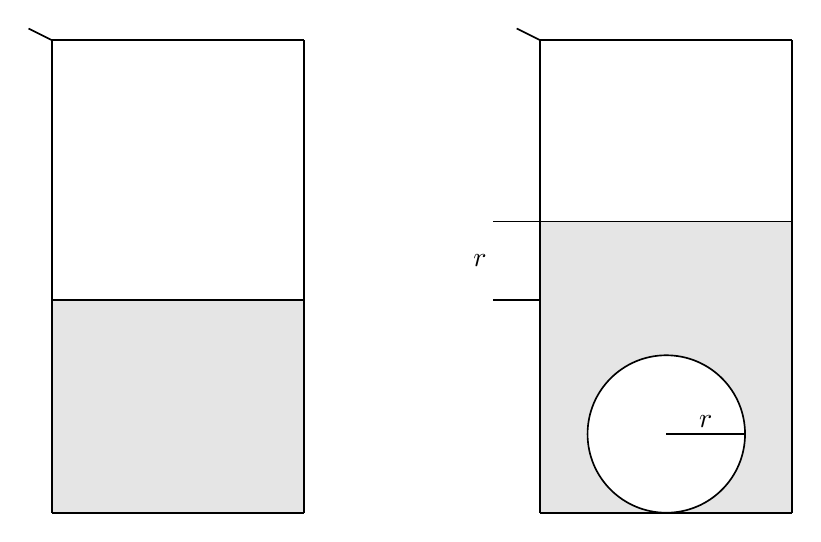
\begin{tikzpicture}[x=1cm,y=1cm,line width=.6pt,font=\normalsize]
% water fills (gray) drawn first
\fill[gray!20] (0,0) rectangle (3.2,2.7);
\fill[gray!20] (6.2,0) rectangle (9.4,3.7);
% ball kept white so water does not cover it
\fill[white] (7.8,1.0) circle[radius=1.0];
% beaker outlines: walls + bottom + top rim + spout lip
\draw (0,0) -- (0,6);
\draw (3.2,0) -- (3.2,6);
\draw (0,0) -- (3.2,0);
\draw (0,6) -- (3.2,6);
\draw (-0.3,6.15) -- (0,6);
\draw (6.2,0) -- (6.2,6);
\draw (9.4,0) -- (9.4,6);
\draw (6.2,0) -- (9.4,0);
\draw (6.2,6) -- (9.4,6);
\draw (5.9,6.15) -- (6.2,6);
% waterlines
\draw (0,2.7) -- (3.2,2.7);
\draw (6.2,3.7) -- (9.4,3.7);
% rise ticks at left of right beaker (old and new levels)
\draw (5.6,2.7) -- (6.2,2.7);
\draw (5.6,3.7) -- (6.2,3.7);
% ball outline tangent to bottom
\draw (7.8,1.0) circle[radius=1.0];
% ball radius line
\draw (7.8,1.0) -- (8.8,1.0);
% labels with clearance, never on lines
\node[above,inner sep=0pt,yshift=2pt] at (8.3,1.0) {$r$};
\node[left,inner sep=0pt,xshift=-2pt] at (5.6,3.2) {$r$};
\end{tikzpicture}
